% !TEX program = xelatex
\documentclass[UTF8,fontset=fandol,a4paper,11pt]{ctexart}
\usepackage[margin=21mm,top=23mm,bottom=22mm,headheight=16pt]{geometry}
\usepackage{amsmath,amssymb,mathtools,bm}
\usepackage{tikz}
\usetikzlibrary{arrows.meta,calc,angles,quotes,patterns}
\usepackage{xcolor,booktabs,array,longtable,enumitem,fancyhdr,needspace}
\usepackage[unicode,hidelinks]{hyperref}
\definecolor{ink}{HTML}{24343C}
\definecolor{accent}{HTML}{166A70}
\definecolor{muted}{HTML}{65747A}
\definecolor{rulegray}{HTML}{D4DDE0}
\definecolor{warm}{HTML}{966037}
\color{ink}
\setlength{\parindent}{2em}
\setlength{\parskip}{4pt}
\linespread{1.12}
\AtBeginDocument{\setlength{\abovedisplayskip}{6pt plus 2pt minus 1pt}
\setlength{\belowdisplayskip}{6pt plus 2pt minus 1pt}
\setlength{\abovedisplayshortskip}{0pt plus 1pt}
\setlength{\belowdisplayshortskip}{4pt plus 1pt}}
\setlist[enumerate]{label=(\arabic*),leftmargin=2.3em,itemsep=3pt,topsep=4pt}
\setlist[itemize]{leftmargin=2em,itemsep=2pt,topsep=4pt}
\allowdisplaybreaks[1]
\setlength{\emergencystretch}{2em}
\setcounter{secnumdepth}{0}
\providecommand{\tightlist}{\setlength{\itemsep}{0pt}\setlength{\parskip}{0pt}}
\ctexset{section={format=\Large\bfseries\color{accent},beforeskip=10pt,afterskip=9pt},
subsection={format=\normalsize\bfseries\color{accent},beforeskip=10pt,afterskip=4pt},
subsubsection={format=\normalsize\bfseries,beforeskip=8pt,afterskip=3pt}}
\pagestyle{fancy}
\fancyhf{}
\fancyhead[L]{\small\color{muted}物理学难题集萃}
% 页眉仅保留书名；版本名称只在封面显示。
\fancyfoot[L]{\small\color{muted}\chapterlabel}
\fancyfoot[R]{\small\thepage}
\renewcommand{\headrulewidth}{0.4pt}
\renewcommand{\footrulewidth}{0pt}
\newcommand{\dd}{\mathop{}\!\mathrm{d}}
\newcommand{\vect}[1]{\bm{#1}}
\newcommand{\tagline}[1]{\noindent{\small\color{muted}#1}\par}
\newcommand{\result}[1]{\begin{equation*}\boxed{#1}\end{equation*}}
\newcommand{\figcaption}[1]{\par\vspace{2pt}{\small\color{muted}#1}\par}
\newcommand{\teach}[2]{\Needspace{4\baselineskip}\subsection*{讲解要点与追问}#1\par\smallskip\noindent\textbf{追问：}#2\par}
\newcommand{\workarea}{\par\vspace{7mm}\noindent{\small\color{muted}作答区}\par\vspace{4mm}
\noindent\textcolor{rulegray}{\rule{\linewidth}{0.3pt}}\par\vspace{16mm}
\noindent\textcolor{rulegray}{\rule{\linewidth}{0.3pt}}\par\vspace{16mm}
\noindent\textcolor{rulegray}{\rule{\linewidth}{0.3pt}}\par\vspace{16mm}
\noindent\textcolor{rulegray}{\rule{\linewidth}{0.3pt}}}
\tikzset{axis/.style={-{Stealth[length=2mm]},thin,color=muted},
motion/.style={-{Stealth[length=2.3mm]},thick,color=accent},
force/.style={-{Stealth[length=2.3mm]},thick,color=warm},
traj/.style={thick,color=accent},guide/.style={dashed,thin,color=muted},
object/.style={thick,color=ink},every node/.style={font=\small}}\widowpenalty=10000\clubpenalty=10000\displaywidowpenalty=10000\newcommand{\chapterlabel}{热学试题（二）}







\hypersetup{pdftitle={热学试题（二）·学生版},pdfauthor={}}

\begin{document}\pdfbookmark[0]{热学试题（二）}{cover}

\thispagestyle{empty}\vspace*{22mm}

\noindent{\Huge\bfseries 物理学难题集萃}\par\vspace{12mm}

\noindent{\LARGE 热学试题（二）}\par\vspace{12mm}

\noindent{\Large\color{accent}学生版}\par\vspace{9mm}

\noindent\textcolor{accent}{\rule{\linewidth}{1pt}}\par\vspace{9mm}

\noindent 第1--5题\par\vfill\clearpage

\pdfbookmark[1]{题目目录}{contents}\section*{题目目录}

\begin{longtable}{@{}r p{113mm} r@{}}\toprule 题号 & 题目 & 页码\\\midrule

\hyperref[q:1]{1} & \hyperref[q:1]{热容量阶跃下的矩形循环} & \pageref{q:1} \\

\hyperref[q:2]{2} & \hyperref[q:2]{有限热源的最大作功与相变卡诺循环} & \pageref{q:2} \\

\hyperref[q:3]{3} & \hyperref[q:3]{从活塞与分子碰撞导出绝热方程} & \pageref{q:3} \\

\hyperref[q:4]{4} & \hyperref[q:4]{导热稳态、分子扩散与撤热源后的平衡} & \pageref{q:4} \\

\hyperref[q:5]{5} & \hyperref[q:5]{光子气体的压强、绝热关系与辐射能流} & \pageref{q:5} \\

\bottomrule\end{longtable}

\clearpage

\pdfbookmark[2]{第 1 题 热容量阶跃下的矩形循环}{q1}

\section*{第 1 题\quad 热容量阶跃下的矩形循环}\label{q:1}


$\nu$ mol理想气体的定体摩尔热容量为
\[
C_V(T)=
\begin{cases}
\alpha R,&T<2T_0,\\
\alpha\beta R,&T>2T_0,
\end{cases}
\qquad \alpha>1,\quad\beta>1.
\]
气体内能由给定热容量连续积分确定，取$U(0)=0$。气体经历图热试2.1所示的顺时针矩形循环$A\to B\to C\to D\to A$，其中$AB,CD$等体，$BC,DA$等压，已知$T_A=T_0,T_B=2T_0,T_C=3T_0$。
\begin{enumerate}
\item 求$T_D$，画$U$--$T$关系，并在图中标出四态及$CD$上$T=2T_0$的状态$E$。
\item 求循环效率；说明热容量的阶跃是否足以引入定温吸放热。
\end{enumerate}


\begin{center}\begin{minipage}{.98\linewidth}\centering
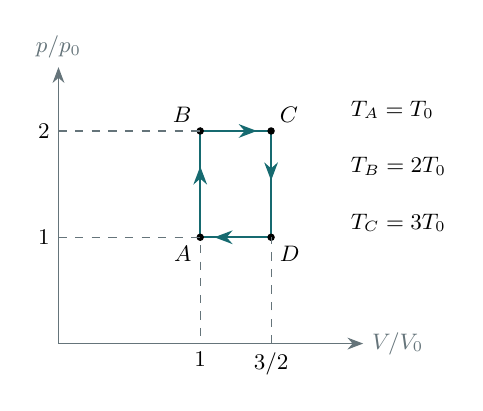
\begin{tikzpicture}[scale=.9,transform shape]

\draw[axis] (0,0)--(4.3,0) node[right] {$V/V_0$};
\draw[axis] (0,0)--(0,3.9) node[above] {$p/p_0$};
\draw[traj] (2,1.5)--(2,3)--(3,3)--(3,1.5)--cycle;
\draw[motion] (2,1.9)--(2,2.5);
\draw[motion] (2.2,3)--(2.8,3);
\draw[motion] (3,2.7)--(3,2.3);
\draw[motion] (2.8,1.5)--(2.2,1.5);
\foreach \x/\y/\lab/\pos in {2/1.5/A/below left,2/3/B/above left,3/3/C/above right,3/1.5/D/below right}{
\fill (\x,\y) circle (1.5pt) node[\pos] {$\lab$};}
\node[below] at (2,0) {$1$};\node[below] at (3,0) {$3/2$};
\node[left] at (0,1.5) {$1$};\node[left] at (0,3) {$2$};
\draw[guide] (0,1.5)--(2,1.5)--(2,0);
\draw[guide] (0,3)--(2,3);\draw[guide] (3,0)--(3,1.5);

\node[right] at (4,3.3) {$T_A=T_0$};
\node[right] at (4,2.5) {$T_B=2T_0$};
\node[right] at (4,1.7) {$T_C=3T_0$};

\end{tikzpicture}
\figcaption{图热试2.1\quad 顺时针矩形循环；体积与压强坐标按初态归一化。}
\end{minipage}\end{center}

\par\vspace{5mm}\noindent{\small\color{muted}作答区}\par\vspace{3mm}\noindent\textcolor{rulegray}{\rule{\linewidth}{0.3pt}}\par\vspace{12mm}\noindent\textcolor{rulegray}{\rule{\linewidth}{0.3pt}}

\clearpage

\pdfbookmark[2]{第 2 题 有限热源的最大作功与相变卡诺循环}{q2}

\section*{第 2 题\quad 有限热源的最大作功与相变卡诺循环}\label{q:2}


两个物体的初温为$T_1>T_2>0$，各自热容量均为常量$C$。以小型可逆热机在两者之间连续工作，每轮换热足够少，可忽略一轮内部热源温度的变化；整体与外界绝热。
\begin{enumerate}
\item 求热机对外总作功的最大值和最终共同温度。
\item 第一轮工质为$\nu$ mol。高温等温过程从$T_1$下的全液态开始，等温等压吸热$L$后全部汽化为体积$V_1$的气体，再在$T_1$等温膨胀至$V_2$。随后经可逆绝热及$T_2$等温过程返回初态。气相除两相共存区外可视为理想气体。定性画出一种能闭合的$p$--$V$和$T$--$S$循环，求第一轮功。这里$L$为全部工质汽化吸收的总潜热。
\end{enumerate}


\begin{center}\begin{minipage}{.98\linewidth}\centering
\begin{tikzpicture}[scale=.9,transform shape]

\draw[object,fill=warm!8] (0,2.8) rectangle (2,4);
\draw[object,fill=accent!8] (0,-.4) rectangle (2,.8);
\draw[object,fill=muted!8] (3.5,1.2) rectangle (5.3,2.4);
\node[align=center] at (1,3.4) {热物体\\$T_1,C$};
\node[align=center] at (1,.2) {冷物体\\$T_2,C$};
\node at (4.4,1.8) {可逆热机};
\draw[force] (2,3.4)--(4.4,3.4)--(4.4,2.45);
\node[above] at (3.2,3.4) {$Q_h$};
\draw[force] (4.4,1.15)--(4.4,.2)--(2,.2);
\node[below] at (3.2,.2) {$Q_c$};
\draw[motion] (5.35,1.8)--(6.8,1.8) node[right] {$W$};
\draw[guide,rounded corners] (-.3,-.7) rectangle (6,4.3);
\node[below] at (2.8,-.8) {整体绝热，仅向外输出功};

\end{tikzpicture}
\figcaption{图热试2.2\quad 两物体温度随连续微小循环改变，整体能量减少量为输出功。}
\end{minipage}\end{center}

\par\vspace{5mm}\noindent{\small\color{muted}作答区}\par\vspace{3mm}\noindent\textcolor{rulegray}{\rule{\linewidth}{0.3pt}}\par\vspace{12mm}\noindent\textcolor{rulegray}{\rule{\linewidth}{0.3pt}}

\clearpage

\pdfbookmark[2]{第 3 题 从活塞与分子碰撞导出绝热方程}{q3}

\section*{第 3 题\quad 从活塞与分子碰撞导出绝热方程}\label{q:3}


理想气体封闭在柱形绝热气缸中，一端为密封、无摩擦的刚性活塞。将活塞缓慢推入气缸，分子与活塞作弹性碰撞，获得的能量经分子碰撞重新分配到各自由度。
利用这一微观模型导出气体准静态绝热过程的$T$--$V$关系，设摩尔热容量$C_V$及$\gamma=C_p/C_V$为常量。须给出碰撞通量、单分子能量变化和速度分布积分，并说明“缓慢”怎样进入近似。


\begin{center}\begin{minipage}{.98\linewidth}\centering
\begin{tikzpicture}[scale=.9,transform shape]

\draw[object] (0,2.2)--(0,0)--(5.5,0);
\draw[object] (0,2.2)--(5.5,2.2);
\fill[accent!7] (.03,.03) rectangle (4.5,2.17);
\draw[object,line width=2pt] (4.5,0)--(4.5,2.2);
\draw[object] (4.5,1.1)--(6,1.1);
\draw[motion] (5.7,1.6)--(4.7,1.6) node[midway,above] {$-u\hat x$};
\fill (2.6,1.4) circle (2pt);
\draw[motion] (2.6,1.4)--(3.7,1.4) node[midway,above] {$v_x$};
\draw[axis] (0,-.45)--(6,-.45) node[right] {$x$};
\node at (2, .6) {$n,\ T,\ m$};
\node[above] at (2.3,2.35) {绝热壁};

\end{tikzpicture}
\figcaption{图热试2.3\quad 活塞在右端向左推进，气体分子朝右迎撞。}
\end{minipage}\end{center}

\workarea

\clearpage

\pdfbookmark[2]{第 4 题 导热稳态、分子扩散与撤热源后的平衡}{q4}

\section*{第 4 题\quad 导热稳态、分子扩散与撤热源后的平衡}\label{q:4}


侧面绝热的柱形容器由长度$L$的均匀固体分隔成等体积区域1、2，两区装相同分子的理想气体，区域1的气体质量为区域2的两倍。固体不能移动，热膨胀忽略，导热系数与横截面积均为常量。两区分别由温度$T_1$与$T_2>T_1$的热源维持温度，忽略各气区内部温差，已达到导热稳态。
\begin{enumerate}
\item 求固体沿轴向的温度分布，取左端$x=0$、右端$x=L$。
\item 同时跟踪两区各一个分子，时间$t$远长于平均碰撞间隔，但跟踪期间未遇容器壁。求其离初始点的典型距离之比，以均方根位移$R_{i,\rm rms}=\sqrt{\langle|\boldsymbol R_i|^2\rangle}$表示；并说明这个统计比值与单次轨迹距离比的关系。
\item 定体摩尔热容量$C_V$为常量，区域2有$\nu_2$ mol气体。固体有$\nu_s$ mol、摩尔热容量$C_s$，满足$\nu_sC_s=2\nu_2C_V$。撤去两热源，使整体与外界绝热，求最终共同温度。
\end{enumerate}
第（2）问采用各向同性随机飞行近似：相邻自由程方向独立、长度服从均值$\lambda$的指数分布，平均速率$\bar v\propto\sqrt T$，相同硬球分子的$\lambda\propto1/n$。


\begin{center}\begin{minipage}{.98\linewidth}\centering
\begin{tikzpicture}[scale=.9,transform shape]

\draw[object] (0,0) rectangle (7,2.2);
\fill[accent!8] (.03,.03) rectangle (2.3,2.17);
\fill[muted!12] (2.3,.03) rectangle (4.7,2.17);
\fill[warm!8] (4.7,.03) rectangle (6.97,2.17);
\draw[object] (2.3,0)--(2.3,2.2);\draw[object] (4.7,0)--(4.7,2.2);
\node[align=center] at (1.15,1.1) {区域1\\$T_1,\ 2\nu_2$};
\node[align=center] at (3.5,1.1) {固体\\$\nu_sC_s$};
\node[align=center] at (5.85,1.1) {区域2\\$T_2,\ \nu_2$};
\draw[axis] (2.3,-.6)--(5.2,-.6) node[right] {$x$};
\node[below] at (2.3,-.6) {$0$};\node[below] at (4.7,-.6) {$L$};
\node[above] at (3.5,2.4) {侧面绝热；$T_2>T_1$};

\end{tikzpicture}
\figcaption{图热试2.4\quad 两气区体积相等，固体温度由左右热源维持。}
\end{minipage}\end{center}

\par\vspace{5mm}\noindent{\small\color{muted}作答区}\par\vspace{3mm}\noindent\textcolor{rulegray}{\rule{\linewidth}{0.3pt}}\par\vspace{12mm}\noindent\textcolor{rulegray}{\rule{\linewidth}{0.3pt}}

\clearpage

\pdfbookmark[2]{第 5 题 光子气体的压强、绝热关系与辐射能流}{q5}

\section*{第 5 题\quad 光子气体的压强、绝热关系与辐射能流}\label{q:5}


黑体空腔的热辐射视为光子气体。频率为$\nu$的光子能量$\varepsilon=h\nu$、动量大小$p_\gamma=h\nu/c$；按频段记数密度$n_\nu$、能量密度$u_\nu=n_\nu h\nu$，总能量密度$u=\sum_\nu u_\nu$。光子静质量为零。热平衡时速度大小均为$c$，方向各向同性。
\begin{enumerate}
\item 先将壁面视为理想反射面，证明辐射压强$p=u/3$。
\item 对充分热化的黑体辐射，结合热力学第二定律说明$u$与壁材、腔体体积无关，只依赖温度，并导出$u=aT^4$。采用忽略表面与有限尺寸效应的宏观腔体近似。
\item 导出准静态可逆绝热过程中$p$与体积$V$的关系。
\item 求任意一光子的$x$方向速度分量分布$f(v_x)$。
\item 在壁上开一个不扰动内部平衡的小孔，证明单位孔面积的向外辐射功率$J=cu/4$，由此给出$J$随温度的规律。
\end{enumerate}
可用热力学恒等式
\[
\left(\frac{\partial U}{\partial V}\right)_T
=T\left(\frac{\partial p}{\partial T}\right)_V-p.
\]
空腔在求平衡态时允许吸收、发射以充分热化；反射面用于计算瞬时动量传递和理想绝热过程。


\begin{center}\begin{minipage}{.98\linewidth}\centering
\begin{tikzpicture}[scale=.9,transform shape]

\draw[object,fill=accent!4] (0,0) rectangle (6,3.6);
\draw[motion] (1,2.6)--(6,.8);
\draw[motion] (6,.8)--(3.77777778,0);
\draw[motion] (4.4,2.9)--(5.8,2.1);
\draw[motion] (1.1,.5)--(.15,1.8);
\draw[axis] (6,1.8)--(7.5,1.8) node[right] {$+\hat x$};
\node[align=center] at (2.2,3.1) {各向同性热辐射};
\node at (3,-1) {$\varepsilon=h\nu,\quad p_\gamma=\varepsilon/c$};
\node[below] at (3,-.2) {充分热化的宏观空腔};

\end{tikzpicture}
\figcaption{图热试2.5\quad 以腔壁法线定义x方向，光子方向各向同性。}
\end{minipage}\end{center}

\par\vspace{5mm}\noindent{\small\color{muted}作答区}\par\vspace{3mm}\noindent\textcolor{rulegray}{\rule{\linewidth}{0.3pt}}\par\vspace{12mm}\noindent\textcolor{rulegray}{\rule{\linewidth}{0.3pt}}

\end{document}
